\section{Durchführung}
\label{sec:Durchführung}
Um die Zeitabhängigkeit der Amplitude zu untersuchen wurde der Versuch wie in Abbildung \ref{fig:aufb a} aufgebaut.
\begin{figure}
    \centering
    \caption{Aufbau zur Untersuchung einer ungedämften und erzwungenen Schwingung \cite{v354}} 
    \label{fig:aufb a}
    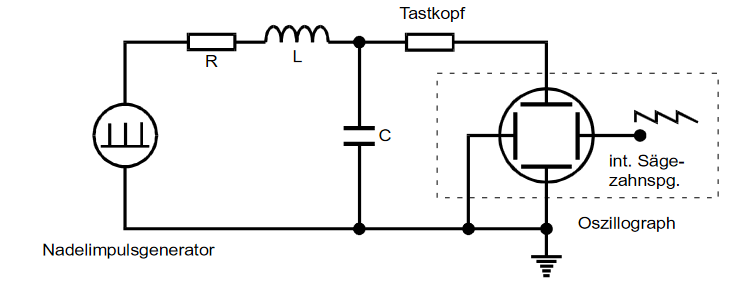
\includegraphics[width = 0.5\textwidth]{pics/aufb.png}
\end{figure}
Dabei wurde an Stelle des Nadelimpulsgenerators ein Rechtecksignal genutzt. 
Der RLC-Kreis wird mit niederfrequenten Rechteckimpulsen ausgelegt und zum Schwingen angeregt.
Es werden die Amplituden der Spannung $U_\text{C}$ in Abhängigkeit von der Zeit $t$ der gedämpften Schwingung ausgelesen und notiert.
\\
Der Durchführung des zweiten Versuchsteils erfolgt mit dem selben Aufbau wie in Abbildung \ref{fig:aufb a}.
Jedoch wird der Widerstand durch einen verstellbaren ersetzt. Dann wird versucht durch variation des Widerstands den aperiodischen Grenzfall zu erreichen.
Sobald dieser erreicht ist wird der Wert für den Widerstand notiert.
\\
Für den dritten Versuchsteil wurde erneut der Versuch wie in Abbildung \ref{fig:aufb a} aufgebaut. Dieses mal wird aber nur die Rechteckspannung durch eine Sinusspannung ersetzt.
Die Abhängigkeit der Kondensatorspannung $U_\text{C}$ von der Frequenz wird untersucht, indem die Frequenz von $\SI{5}{\kilo \hertz}$ bis $\SI{60}{\kilo \hertz}$ erhöht wird.

